\begin{figure}[t]
\centering
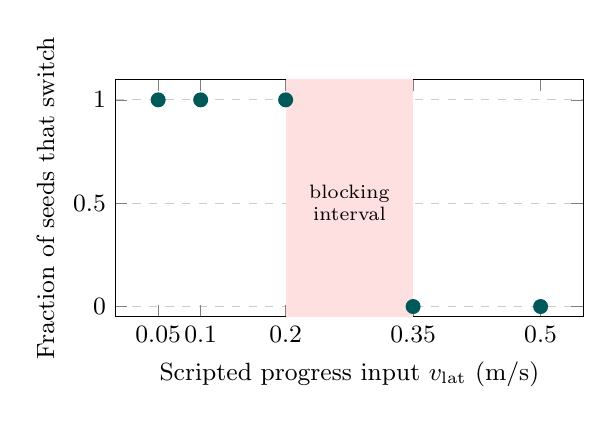
\begin{tikzpicture}
\begin{axis}[
  width=0.62\linewidth, height=4.6cm,
  xmin=0, xmax=0.55, ymin=-0.05, ymax=1.1,
  xlabel={Scripted progress input $v_{\mathrm{lat}}$ (m/s)},
  ylabel={Fraction of seeds that switch},
  xtick={0.05,0.10,0.20,0.35,0.50},
  xticklabel style={/pgf/number format/fixed, /pgf/number format/precision=2},
  ymajorgrids, grid style={dashed,gray!40},
  tick label style={font=\small}, label style={font=\small},
]
\fill[red!12] (axis cs:0.20,-0.05) rectangle (axis cs:0.35,1.1);
\node[font=\scriptsize,align=center] at (axis cs:0.275,0.5) {blocking\\interval};
\addplot[only marks, mark=*, mark size=2.5pt, teal!70!black] coordinates {(0.05,1.00) (0.10,1.00) (0.20,1.00) (0.35,0.00) (0.50,0.00)};
\end{axis}
\end{tikzpicture}
\caption{\textbf{Offline transition blocking under fast progress saturation} (\texttt{clean\_commit}, Full, 50 seeds per point, measured only at the five marked inputs; data from \texttt{R5\_rho\_sweep.md}). Every seed commits the warranted switch for $v_{\text{lat}}\le0.20$~m/s and none does for $v_{\text{lat}}\ge0.35$~m/s, so the transition-blocking interval is $v_{\text{lat}}\in(0.20,0.35)$~m/s. This is a sensitivity of the scripted progress input, not a physical freezing threshold.}
\label{fig:rhosweep}
\end{figure}
